%definira klasu dokumenta 
\documentclass[12pt]{report} 

%prostor izmedu naredbi \documentclass i \begin{document} se zove uvod. U njemu se nalaze naredbe koje se odnose na cijeli dokument

%osnovni LaTex ne može riješiti sve probleme, pa se koriste različiti paketi koji olakšavaju izradu željenog dokumenta
\usepackage[croatian]{babel} 
\usepackage{amssymb}
\usepackage{amsmath}
\usepackage{txfonts}
\usepackage{mathdots}
\usepackage{titlesec}
\usepackage{array}
\usepackage{lastpage}
\usepackage{etoolbox}
\usepackage{tabularray}
\usepackage{color, colortbl}
\usepackage{adjustbox}
\usepackage{geometry}
\usepackage[classicReIm]{kpfonts}
\usepackage{hyperref}
\usepackage{fancyhdr}

\usepackage{float}
\usepackage{setspace}
\restylefloat{table}


\patchcmd{\chapter}{\thispagestyle{plain}}{\thispagestyle{fancy}}{}{} %redefiniranje stila stranice u paketu fancyhdr

%oblik naslova poglavlja
\titleformat{\chapter}{\normalfont\huge\bfseries}{\thechapter.}{20pt}{\Huge}
\titlespacing{\chapter}{0pt}{0pt}{40pt}


\linespread{1.3} %razmak između redaka

\geometry{a4paper, left=1in, top=1in,}  %oblik stranice

\hypersetup{ colorlinks, citecolor=black, filecolor=black, linkcolor=black,	urlcolor=black }   %izgled poveznice


%prored smanjen između redaka u nabrajanjima i popisima
\newenvironment{packed_enum}{
	\begin{enumerate}
		\setlength{\itemsep}{0pt}
		\setlength{\parskip}{0pt}
		\setlength{\parsep}{0pt}
	}{\end{enumerate}}

\newenvironment{packed_item}{
	\begin{itemize}
		\setlength{\itemsep}{0pt}
		\setlength{\parskip}{0pt}
		\setlength{\parsep}{0pt}
	}{\end{itemize}}

%boja za privatni i udaljeni kljuc u tablicama
\definecolor{LightBlue}{rgb}{0.9,0.9,1}
\definecolor{LightGreen}{rgb}{0.9,1,0.9}

%Promjena teksta za dugačke tablice
\DefTblrTemplate{contfoot-text}{normal}{Nastavljeno na idućoj stranici}
\SetTblrTemplate{contfoot-text}{normal}
\DefTblrTemplate{conthead-text}{normal}{(Nastavljeno)}
\SetTblrTemplate{conthead-text}{normal}
\DefTblrTemplate{middlehead,lasthead}{normal}{Nastavljeno od prethodne stranice}
\SetTblrTemplate{middlehead,lasthead}{normal}

%podesavanje zaglavlja i podnožja

\pagestyle{fancy}
\lhead{Programsko inženjerstvo}
\rhead{BytePit}
\lfoot{Koder kolege}
\cfoot{stranica \thepage/\pageref{LastPage}}
\rfoot{\today}
\renewcommand{\headrulewidth}{0.2pt}
\renewcommand{\footrulewidth}{0.2pt}


\begin{document} 
	
	
	
	\begin{titlepage}
		\begin{center}
			\vspace*{\stretch{1.0}} %u kombinaciji s ostalim \vspace naredbama definira razmak između redaka teksta
			\LARGE Programsko inženjerstvo\\
			\large Ak. god. 2023./2024.\\
			
			\vspace*{\stretch{3.0}}
			
			\huge $$BytePit$$\\
			\Large Dokumentacija, Rev. \textit{1}\\
			
			\vspace*{\stretch{12.0}}
			\normalsize
			Grupa: \textit{Koder kolege}\\
			Voditelj: \textit{Petra Kelković}\\
			
			
			\vspace*{\stretch{1.0}}
			Datum predaje: \textit{17. studenoga 2023.}\\
	
			\vspace*{\stretch{4.0}}
			
			Nastavnik: \textit{Hrvoje Nuić}\\
		
		\end{center}

	
	\end{titlepage}

	
	\tableofcontents


	\chapter{Dnevnik promjena dokumentacije}
		
		\textbf{\textit{Kontinuirano osvježavanje}}\\
				
		
		\begin{longtblr}[
				label=none
			]{
				width = \textwidth, 
				colspec={|X[2]|X[13]|X[3]|X[3]|}, 
				rowhead = 1
			}
			\hline
			\textbf{Rev.}	& \textbf{Opis promjene/dodatka} & \textbf{Autori} & \textbf{Datum}\\[3pt] \hline
			0.1 & Personalizirana naslovna stranica \newline te header i footer.	& Dora Bilić-Pavlinović & 28.10.2023.		\\[3pt] \hline 
			0.2.1	& Opis projektnog zadatka - opći opis & Dora Bilić-Pavlinović & 28.10.2023. 	\\[3pt] \hline 
			0.2.2	& Opis projektnog zadatka - slične aplikacije i druge primjene  & Matea Cvetković & 29.10.2023. 	\\[3pt] \hline
			0.2.3 & Opis projektnog zadatka - final touches & Filip \newline Mohler & 31.10.2023. 	\\[3pt] \hline
			0.3.1	& Funkcijski zahtjevi & Petra \newline Kelković, \newline Mislav Korotaj & 30.10.2023. 	\\[3pt] \hline 
			0.4.1	& Obrasci upotrebe (UC dijagrami) - prvi dio & Mislav Korotaj & 31.10.2023. 	\\[3pt] \hline 
			0.4.2	& Obrasci upotrebe - drugi dio & Mislav Korotaj, \newline Nives Ostojić, \newline Filip Mohler & 31.10.2023. 	\\[3pt] \hline 
			0.4.3 & Obrasci upotrebe - treći dio & Filip \newline Mohler & 3.11.2023. 	\\[3pt] \hline
			0.4.4 & Obrasci upotrebe - dijagrami & Filip \newline Mohler & 6.11.2023. 	\\[3pt] \hline
			0.5.1 & Sekvencijski dijagrami & Petra Buršić & 
			6.11.2023. \\[3pt] \hline 
			0.5.2 & Sekvencijski dijagrami - nastavak & Petra Buršić & 7.11.2023. \\[3pt] \hline 
			0.5.3. & Sekvencijski dijagrami - finalno & Petra Buršić & 10.11.2023. \\[3pt] \hline 
			0.6 & Unos sastanka: podjela uloga\newline Plan daljnjeg rada & svi & 20.10.2023. \\[3pt] \hline 
			0.7 & Opis arhitekture sustava i baze podataka & Nives \newline Ostojić & 10.11.2023. \\[3pt] \hline 
			0.8 & Ispravak sekvencijskih dijagrama \newline
			Dodani ostali zahtjevi & Filip \newline Mohler & 13.11.2023. \\[3pt] \hline 
			0.9 &Popravljena dokumentacija na sastanku & svi & 
			14.11.2023. \\[3pt] \hline 
			0.10 & Dijagrami razreda + opis & Matea Cvetković & 15.11.2023. \\[3pt] \hline 
			0.11 & ER dijagram baze i opis & Filip \newline Mohler & 16.11.2023. \\[3pt] \hline 
			\textbf{1.0} & Verzija samo s bitnim dijelovima za 1. ciklus & * & 16.11.2023. \\[3pt] \hline 
		\end{longtblr}
	
	\chapter{Opis projektnog zadatka}
		
		
		
		Tema našeg projektnog rada je izrada web aplikacije \textit{"BytePit"} koja omogućuje korisnicima sudjelovanje u programerskim natjecanjima i provjeru riješenih zadataka. Ideja je da naša stranica ima sve potrebno za obavljanje natjecanja poput registracije korisnika, uključivanje u natjecanje, pribavljanje zadataka, vrjednovanje priloženih rješenja, prikaz dosadašnjih uspjeha natjecatelja i još mnogo toga.
	
		Neregistrirani korisnik može se registrirati definirajući registrira li se kao \textbf{voditelj} ili \textbf{natjecatelj}
		Za registraciju korisnika potrebno je  unjeti \begin{packed_item}
			\item korisničko ime
			\item fotografiju
			\item lozinku
			\item ime
			\item prezime
			\item email adresu
		\end{packed_item}
		Upješnost registracije potvrđuje se preko email adrdese dok dodatno voditelja potvrđuje i administrator.
		
		\textbf{\textit{Neregistrirani korisnik}} na web stranici može vidjeti kalendar s natjecanjima kojima je moguće pristupiti te pregledati zadatke na stranici. Također, omogućen mu je uvid u profile natjecatelja i voditelja. Svi registrirani korisnici automatski nasljeđuju sve ove mogućnosti koje neregistrirani korisnici imaju.
		
	    \textbf{\textit{Natjecatelj}} prisustuje natjecanjima te dobiva uvid u svoje rezultate. U svrhu pripreme za spomenuta natjecanja, na stranici su dostupni zadatci za vježbu te je dostupna opcija virtualnog natjecanja.
	    
	    \textbf{\textit{Voditelj}} ima veće ovlasti od natjecatelja. U njegovim rukama leži zadatak učitavanja novih zadataka na web aplikaciju te organizacija natjecanja. Kada voditelj izradi natjecanje, ono postaje vidljivo u kalendaru dostupnom natjecateljima. Dakle, zadatak voditelja je odrediti težinu natjecateljskog ispita, broj zadataka i dostupno vrijeme za rješavanje istih te postavljanje termina ispita. Ukoliko želi, voditelj može učitati sličicu pehara.  
	    
	    \textbf{\textit{Administrator}} ima, naravno, najviše ovlasti među navedenima. On može vidjeti popis svih registriranih korisnika zajedno s njihovim osobnim podatcima te im on onda dodjeljuje prava i po potrebi mijenja osobne podatke. Također, može uređivati sve zadatke i natjecanja koja su voditelji postavili na aplikaciju. Administratorova dužnost je ne zloupotrebljavati osobne podatke korisnika, što je i kažnjivo zakonom.
	    
	    Na profilu natjecatelja prikazana je statistička obrada njegovih dosadašnjih uspjeha. Stoga mu na profilu možemo vidjeti koliko je zadataka uspješno riješio a koliko ih je pokušavao riješiti te koliko je natjecanja osvojio. Za svako osvojeno natjecanje, na profilu će mu biti prikazana po jedna slikica pehara.
	    Profil voditelja prikazuje popis zadataka koje je on učitao te natjecanja koje je on organizirao. \\
	
		\noindent{\Large {Provedba natjecanja}}\\
		Kada dođe vrijeme koje je voditelj postavio kao početak natjecanja, zadatci ispita postaju vidljivi aktivnim natjecateljima. Za svaki zadatak natjecatelji prilažu datoteke s programskim kodom. Na ispitu stoje postavljena vremenska ograničenja za trajanje ispita i nakon njegovog isteka objavljuju se rezultati. Rezultati se prikazuju oblikom rang liste svih učesnika poredanih silazno po prikupljenom broju bodova. Pri kalkulaciji broja bodova uzima se u obzir postotak točnosti i isteklo vrijeme. Onima koji su se plasirali na prva tri mjesta pridodaje se slika pehara na njihovom profilu.
		Natjecatelju je po završetku ispita pridodan i uvid u sva priložena rješenja nekog drugog natjecatelja. Također, može vidjeti statistiku svakog pojedinog zadatka uključujući prosječno vrijeme rješavanja, popis natjecatelja koji su ga rješavali i sl.
		
		
		\noindent{\Large {Virtualno natjecanje}}\\
		Virtualno natjecanje je koncept osmišljen kako bi natjecatelji mogli provjeriti koliko su se dobro pripremili za nadolazeće natjecanje. Dakle, kada korisnik želi provjeriti svoju spremnost samo ode u kalendar, odabere neko natjecanje koje je provedeno u prošlosti te pokrene virtualno natjecanje and njim. Tada će iz korisnikove perspective sve izgledati kao da on sudjeluje na tom natjecanju. Bit će mu pružen isti ispit I po završetku rješavanja biti će rangiran među natjecateljima koji su taj ispit službeno rješavali. Korisnik tako dobiva informaciju kakav bi bio njegov rezultat da je taj dan uistinu sudjelovao na natjecanju.\\
		\noindent{\Large {Slične str,korisnost,upotreba str.}}\\
		\eject
		
		
		
		\section{Primjeri u \LaTeX u}
		
		\textit{Ovo potpoglavlje izbrisati.}\\

		U nastavku se nalaze različiti primjeri kako koristiti osnovne funkcionalnosti \LaTeX a koje su potrebne za izradu dokumentacije. Za dodatnu pomoć obratiti se asistentu na projektu ili potražiti upute na sljedećim web sjedištima:
		\begin{itemize}
			\item Upute za izradu diplomskog rada u \LaTeX u - \url{https://www.fer.unizg.hr/_download/repository/LaTeX-upute.pdf}
			\item \LaTeX\ projekt - \url{https://www.latex-project.org/help/}
			\item StackExchange za Tex - \url{https://tex.stackexchange.com/}\\
		
		\end{itemize} 	


		
		\noindent \underbar{podcrtani tekst}, \textbf{podebljani tekst}, 	\textit{nagnuti tekst}\\
		\noindent \normalsize primjer \large primjer \Large primjer \LARGE {primjer} \huge {primjer} \Huge primjer \normalsize
				
		\begin{packed_item}
			
			\item  primjer
			\item  primjer
			\item  primjer
			\item[] \begin{packed_enum}
				\item primjer
				\item[] \begin{packed_enum}
					\item[1.a] primjer
					\item[b] primjer
				\end{packed_enum}
				\item primjer
			\end{packed_enum}
			
		\end{packed_item}
		
		\noindent primjer url-a: \url{https://www.fer.unizg.hr/predmet/proinz/projekt}
		
		\noindent posebni znakovi: \# \$ \% \& \{ \} \_ 
		$|$ $<$ $>$ 
		\^{} 
		\~{} 
		$\backslash$ 
		
		
		\begin{longtblr}[
			label=none,
			entry=none
			]{
				width = \textwidth,
				colspec={|X[8,l]|X[8, l]|X[16, l]|}, 
				rowhead = 1,
			} %definicija širine tablice, širine stupaca, poravnanje i broja redaka naslova tablice
			\hline \SetCell[c=3]{c}{\textbf{naslov unutar tablice}}	 \\ \hline[3pt]
			\SetCell{LightGreen}IDKorisnik & INT	&  	Lorem ipsum dolor sit amet, consectetur adipiscing elit, sed do eiusmod  	\\ \hline
			korisnickoIme	& VARCHAR &   	\\ \hline 
			email & VARCHAR &   \\ \hline 
			ime & VARCHAR	&  		\\ \hline 
			\SetCell{LightBlue} primjer	& VARCHAR &   	\\ \hline 
		\end{longtblr}
		

		\begin{longtblr}[
				caption = {Naslov s referencom izvan tablice},
				entry = {Short Caption},
			]{
				width = \textwidth, 
				colspec = {|X[8,l]|X[8,l]|X[16,l]|}, 
				rowhead = 1,
			}
			\hline
			\SetCell{LightGreen}IDKorisnik & INT	&  	Lorem ipsum dolor sit amet, consectetur adipiscing elit, sed do eiusmod  	\\ \hline
			korisnickoIme	& VARCHAR &   	\\ \hline 
			email & VARCHAR &   \\ \hline 
			ime & VARCHAR	&  		\\ \hline 
			\SetCell{LightBlue} primjer	& VARCHAR &   	\\ \hline 
		\end{longtblr}
	


		
		
		%unos slike
		\begin{figure}[H]
			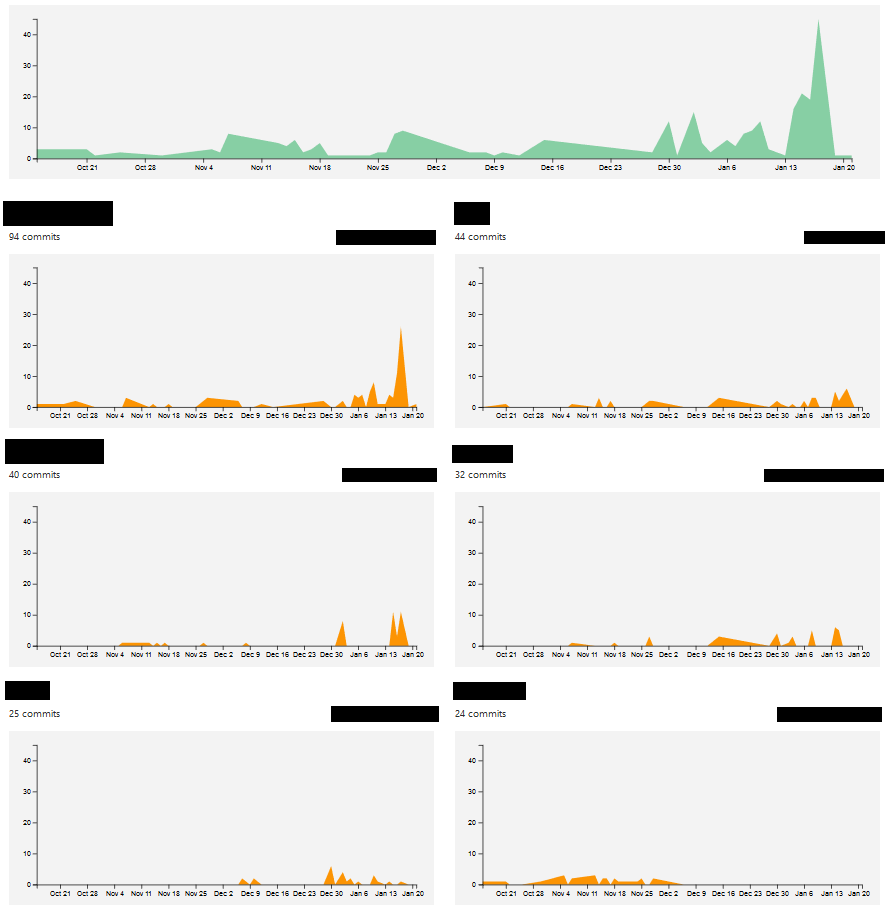
\includegraphics[scale=0.4]{slike/aktivnost.PNG} %veličina slike u odnosu na originalnu datoteku i pozicija slike
			\centering
			\caption{Primjer slike s potpisom}
			\label{fig:promjene}
		\end{figure}
		
		\begin{figure}[H]
			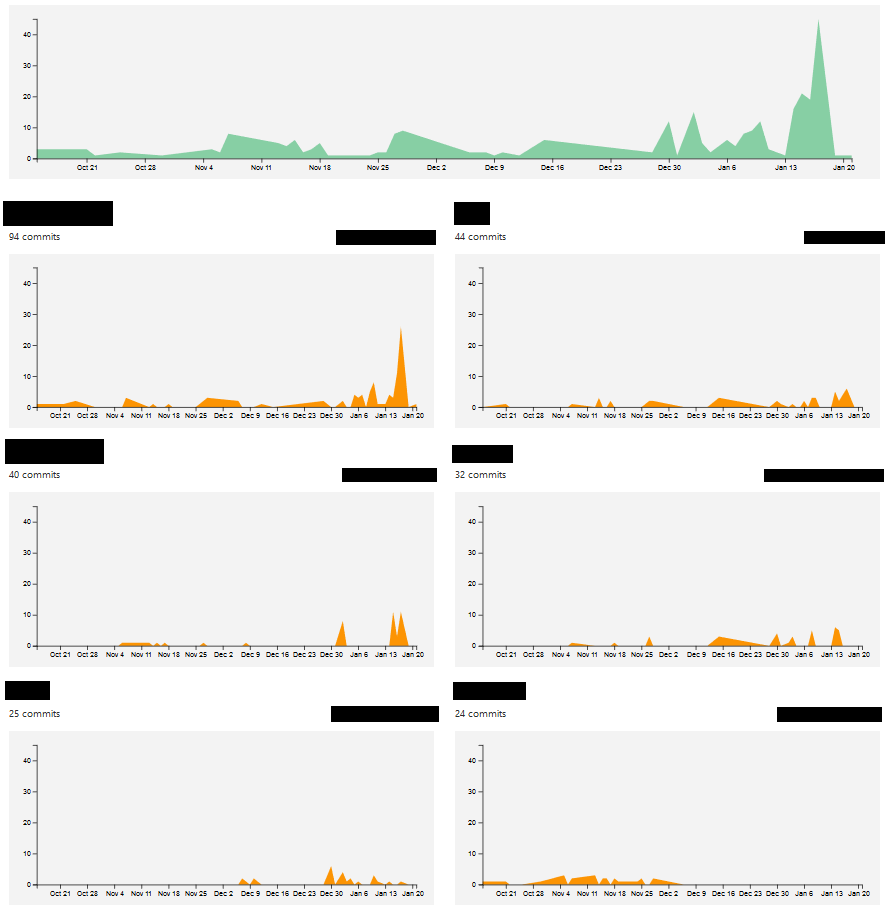
\includegraphics[width=\textwidth]{slike/aktivnost.PNG} %veličina u odnosu na širinu linije
			\caption{Primjer slike s potpisom 2}
			\label{fig:promjene2} %label mora biti drugaciji za svaku sliku
		\end{figure}
		
		Referenciranje slike \ref{fig:promjene2} u tekstu.
		
		\eject
		
	
	\chapter{Specifikacija programske potpore}
		
	\section{Funkcionalni zahtjevi}
			
			\textbf{\textit{dio 1. revizije}}\\
			
			\textit{Navesti \textbf{dionike} koji imaju \textbf{interes u ovom sustavu} ili  \textbf{su nositelji odgovornosti}. To su prije svega korisnici, ali i administratori sustava, naručitelji, razvojni tim.}\\
				
			\textit{Navesti \textbf{aktore} koji izravno \textbf{koriste} ili \textbf{komuniciraju sa sustavom}. Oni mogu imati inicijatorsku ulogu, tj. započinju određene procese u sustavu ili samo sudioničku ulogu, tj. obavljaju određeni posao. Za svakog aktora navesti funkcionalne zahtjeve koji se na njega odnose.}\\
			
			
			\noindent \textbf{Dionici:}
			
			\begin{packed_enum}
				
				\item Dionik 1
				\item Dionik 2				
				\item ...
				
			\end{packed_enum}
			
			\noindent \textbf{Aktori i njihovi funkcionalni zahtjevi:}
			
			
			\begin{packed_enum}
				\item  \underbar{Aktor 1 (inicijator) može:}
				
				\begin{packed_enum}
					
					\item funkcionalnost 1
					\item funkcionalnost 2
					\begin{packed_enum}
						
						\item  podfunkcionalnost 1 
						\item  podfunkcionalnost 2
				
					\end{packed_enum}
					\item  funkcionalnost 3
					
				\end{packed_enum}
			
				\item  \underbar{Aktor 2 (sudionik) može:}
				
				\begin{packed_enum}
					
					\item funkcionalnost 1
					\item funkcionalnost 2
					
				\end{packed_enum}
			\end{packed_enum}
			
			\eject 
			
			
				
			\subsection{Obrasci uporabe}
				
				\textbf{\textit{dio 1. revizije}}
				
				\subsubsection{Opis obrazaca uporabe}
					\textit{Funkcionalne zahtjeve razraditi u obliku obrazaca uporabe. Svaki obrazac je potrebno razraditi prema donjem predlošku. Ukoliko u nekom koraku može doći do odstupanja, potrebno je to odstupanje opisati i po mogućnosti ponuditi rješenje kojim bi se tijek obrasca vratio na osnovni tijek.}\\
					

					\noindent \underbar{\textbf{UC$<$broj obrasca$>$ -$<$ime obrasca$>$}}
					\begin{packed_item}
	
						\item \textbf{Glavni sudionik: }$<$sudionik$>$
						\item  \textbf{Cilj:} $<$cilj$>$
						\item  \textbf{Sudionici:} $<$sudionici$>$
						\item  \textbf{Preduvjet:} $<$preduvjet$>$
						\item  \textbf{Opis osnovnog tijeka:}
						
						\item[] \begin{packed_enum}
	
							\item $<$opis korak jedan$>$
							\item $<$opis korak dva$>$
							\item $<$opis korak tri$>$
							\item $<$opis korak četiri$>$
							\item $<$opis korak pet$>$
						\end{packed_enum}
						
						\item  \textbf{Opis mogućih odstupanja:}
						
						\item[] \begin{packed_item}
	
							\item[2.a] $<$opis mogućeg scenarija odstupanja u koraku 2$>$
							\item[] \begin{packed_enum}
								
								\item $<$opis rješenja mogućeg scenarija korak 1$>$
								\item $<$opis rješenja mogućeg scenarija korak 2$>$
								
							\end{packed_enum}
							\item[2.b] $<$opis mogućeg scenarija odstupanja u koraku 2$>$
							\item[3.a] $<$opis mogućeg scenarija odstupanja  u koraku 3$>$
							
						\end{packed_item}
					\end{packed_item}
				
					
				\subsubsection{Dijagrami obrazaca uporabe}
					
					\textit{Prikazati odnos aktora i obrazaca uporabe odgovarajućim UML dijagramom. Nije nužno nacrtati sve na jednom dijagramu. Modelirati po razinama apstrakcije i skupovima srodnih funkcionalnosti.}
				\eject		
				
			\subsection{Sekvencijski dijagrami}
				
				\textbf{\textit{dio 1. revizije}}\\
				
				\textit{Nacrtati sekvencijske dijagrame koji modeliraju najvažnije dijelove sustava (max. 4 dijagrama). Ukoliko postoji nedoumica oko odabira, razjasniti s asistentom. Uz svaki dijagram napisati detaljni opis dijagrama.}
				\eject
	
		\section{Ostali zahtjevi}
		
			\textbf{\textit{dio 1. revizije}}\\
		 
			 \textit{Nefunkcionalni zahtjevi i zahtjevi domene primjene dopunjuju funkcionalne zahtjeve. Oni opisuju \textbf{kako se sustav treba ponašati} i koja \textbf{ograničenja} treba poštivati (performanse, korisničko iskustvo, pouzdanost, standardi kvalitete, sigurnost...). Primjeri takvih zahtjeva u Vašem projektu mogu biti: podržani jezici korisničkog sučelja, vrijeme odziva, najveći mogući podržani broj korisnika, podržane web/mobilne platforme, razina zaštite (protokoli komunikacije, kriptiranje...)... Svaki takav zahtjev potrebno je navesti u jednoj ili dvije rečenice.}
			 
			 
			 
	
	\chapter{Arhitektura i dizajn sustava}

		\textit{ Arhitektura ima 3 podsustava:}
	\begin{itemize}
		\item 	\textit{Web preglednik}
		\item 	\textit{Web aplikacija na web poslužitelju}
		\item 	\textit{Baza podataka - PostgreSQL }		
	\end{itemize}


{\underline{Web preglednik} je ujedino i prevoditelj koda koji korisniku omogućuje pregledavanje sadržaja web aplikacije i interakciju s istim.}

{\underline{Web poslužitelj} prima HTTP (engl. Hyper
Text Transfer Protocol) zahtjeve od klijenta (preglednika) koji sadrže informacije o tome što klijent traži, kao što su primjerice URL, GET, POST... i vraća dohvaćeni resurs ako ga ima te vraća statusni kod koji daje informacije o uspješnosti zahtjeva.}

{Tehnologije korištene u našoj aplikaciji temelje se na Spring Bootu i Reactu. Aplikacija se sastoji od serverske komponente napisane u Javi (Spring Boot) i klijentske komponente napisane u JavaScriptu (React). Za razvojno okruženje koristimo IntelliJ, a baza koju koristimo za spremanje podataka o registriranim korisnicima i sve informacije o natjecanjima je PostgrSQL.}

{\underline{Web aplikacija} temelji se na arhitekturi Model-View-Controller (MVC). Ova arhitektura omogućuje organizaciju aplikacije u tri ključne komponente:}

\begin{itemize}
    \item \textbf{Model}: Ova komponenta predstavlja poslovnu logiku i podatke aplikacije. Model je implementiran u Java programskom jeziku (Spring Boot) i odgovoran je za upravljanje podacima, komunikaciju s bazom podataka te izračune i obrade podataka.
    
    \item \textbf{View}: Komponenta za prikaz podataka korisnicima. Prikazi se generiraju u Reactu, a omogućuju korisnicima interakciju s aplikacijom putem web preglednika. Prikazi se oblikuju pomoću HTML-a, CSS-a i JavaScripta.
    
    \item \textbf{Controller}: Kontroler je posrednik između Modela i Viewa. Ova komponenta upravlja korisničkim zahtjevima, prima ulazne podatke od korisnika te izvršava odgovarajuće akcije u Modelu. Kontroler također određuje koji prikaz treba biti poslan korisnicima.\\
\end{itemize}	

				
		\section{Baza podataka}
			

			
		{Koristimo relacijsku bazu podataka čije su gradivne jedinke tablice definirane imenom i skupom atributa za jednostavno upravljanje podacima. Baza podataka ove aplikacije sastoji se od sljedećih entiteta:}
	\begin{itemize}
		\item 	\textit{Korisnik}
		\item 	\textit{Natjecanje}
		\item 	\textit{Zadaci na natjecanju}
		\item 	\textit{Zadatak}				
	\end{itemize}
		
			\subsection{Opis tablica}
			

				{\textbf{Korisnik} - entitet sadržava sve važne informacije o korisniku: Korisničko ime, lozinku, ime, prezime, sliku, email, tip korisnika (natjecatelj/voditelj). }
				
				
				\begin{longtblr}[
					label=none,
					entry=none
					]{
						width = \textwidth,
						colspec={|X[6,l]|X[6, l]|X[20, l]|}, 
						rowhead = 1,
					} %definicija širine tablice, širine stupaca, poravnanje i broja redaka naslova tablice
					\hline \SetCell[c=3]{c}{\textbf{Korisnik}}	 \\ \hline[3pt]
					 \SetCell{LightGreen}id & INT	&   jedinstveni identifikator korisnika	\\ \hline
					 \SetCell{LightBlue} username	& VARCHAR &   	izabrano korisničko ime\\ \hline 
					 \SetCell{LightBlue}email & VARCHAR &  e-mail adresa korisnika \\ \hline 
					 name & VARCHAR	&  	ime korisnika	\\ \hline 
					 lastname & VARCHAR	&  	prezime korisnika	\\ \hline 
					 image & BYTEA	&  	slika korisnika	\\ \hline							user-type & VARCHAR & natjecatelj ili voditelj natjecanja \\ \hline
					 password & VARCHAR	&  	šifra korisnika	\\ \hline 
\end{longtblr}


				{\textbf{Natjecanje} - entitet sadržava sve važne informacije o natjecanju: Id natjecanja, vrijeme početka, vrijeme završetka, broj zadataka, id voditelja natjecanja. U odnosu je Many-To-One s entitetom korisnik preko atributa voditelja natjecanja. }
				
				
				\begin{longtblr}[
					label=none,
					entry=none
					]{
						width = \textwidth,
						colspec={|X[6,l]|X[6, l]|X[20, l]|}, 
						rowhead = 1,
					} %definicija širine tablice, širine stupaca, poravnanje i broja redaka naslova tablice
					\hline \SetCell[c=3]{c}{\textbf{Natjecanje}}	 \\ \hline[3pt]
					 \SetCell{LightGreen}id & INT	&   jedinstveni identifikator natjecanja	\\ \hline
					  date-time-of-beginning	& TIMESTAMP &   vrijeme početka natjecanja	\\ \hline 
					 date-time-of-ending	& TIMESTAMP &   vrijeme završetka natjecanja	\\ \hline  
					 competition-maker-id & INT	&  	id voditelja natjecanja	\\ \hline 
	 number-of-problems & INT	&  	broj zadataka u natjecanju	\\ \hline 
				\end{longtblr}

				{\textbf{Zadatak} - entitet sadržava sve važne informacije o zadatku. Sadrži atribute id, trajanje natjecanja, booleanski atribut is-private, broj bodova koje je moguće ostvariti, tip problema, tekst zadatka, naslov i id korisnika koji je napravio zadatak. S entitetom Korisnik je u odnosu Many-To-One preko atributa problem-maker-id.}
				
		\begin{longtblr}[
					label=none,
					entry=none
					]{
						width = \textwidth,
						colspec={|X[6,l]|X[6, l]|X[20, l]|}, 
						rowhead = 1,
					} %definicija širine tablice, širine stupaca, poravnanje i broja redaka naslova tablice
					\hline \SetCell[c=3]{c}{\textbf{Zadatak}}	 \\ \hline[3pt]
					 \SetCell{LightGreen} id & INT	&   jedinstveni identifikator zadatka	\\ \hline
				  \SetCell{LightBlue}problem-maker-id & INT	& identifikator vlasnika zadatka	\\ \hline 
					 duration &  NUMERIC	& trajanje zadatka	\\ \hline 
					 is-private &  BOOLEAN	& provjerava je li zadatak objavljen	\\ \hline 
					 problem-type &  INT	&  ?	\\ \hline 
					text &  VARCHAR	& tekst zadatka	\\ \hline 
					 title &  NUMERIC	& naslov zadatka	\\ \hline 

				\end{longtblr}

				{\textbf{Zadaci na natjecanju} - entitet sadržava sve važne informacije odnosu zadatka i natjecanja na kojem se nalazi. Atributi: id natjecanja i id zadatka }

				
				\begin{longtblr}[
					label=none,
					entry=none
					]{
						width = \textwidth,
						colspec={|X[6,l]|X[6, l]|X[20, l]|}, 
						rowhead = 1,
					} %definicija širine tablice, širine stupaca, poravnanje i broja redaka naslova tablice
					\hline \SetCell[c=3]{c}{\textbf{Zadaci u natjecanju}}	 \\ \hline[3pt]
					 \SetCell{LightBlue}competition-id & INT	&    identifikator natjecanja (natjecanje.id)	\\ \hline
					 \SetCell{LightBlue} problem-id & INT	& identifikator zadatka	(problem.id) \\ \hline 
				\end{longtblr} 


				

				{\textbf{Input-output mapa} - entitet sadržava id zadatka te vrijednost i ključ, odnosno na ovaj način se mapiraju rješenja zadataka. }

				
				\begin{longtblr}[
					label=none,
					entry=none
					]{
						width = \textwidth,
						colspec={|X[6,l]|X[6, l]|X[20, l]|}, 
						rowhead = 1,
					} %definicija širine tablice, širine stupaca, poravnanje i broja redaka naslova tablice
					\hline \SetCell[c=3]{c}{\textbf{Input-output mapa}}	 \\ \hline[3pt]
					 \SetCell{LightGreen}problem-id & INT	&  jedinstveni identifikator zadatka	\\ \hline
					 vrijednost & VARCHAR	& ?  \\ \hline 
					 ključ & VARCHAR	& ?  \\ \hline 
				\end{longtblr}
				
				
			
			\subsection{Dijagram baze podataka}
				\textit{ U ovom potpoglavlju potrebno je umetnuti dijagram baze podataka. Primarni i strani ključevi moraju biti označeni, a tablice povezane. Bazu podataka je potrebno normalizirati. Podsjetite se kolegija "Baze podataka".}
			
			\eject
			
			
		\section{Dijagram razreda}
		
			\textit{Potrebno je priložiti dijagram razreda s pripadajućim opisom. Zbog preglednosti je moguće dijagram razlomiti na više njih, ali moraju biti grupirani prema sličnim razinama apstrakcije i srodnim funkcionalnostima.}\\
			
			\textbf{\textit{dio 1. revizije}}\\
			
			\textit{Prilikom prve predaje projekta, potrebno je priložiti potpuno razrađen dijagram razreda vezan uz \textbf{generičku funkcionalnost} sustava. Ostale funkcionalnosti trebaju biti idejno razrađene u dijagramu sa sljedećim komponentama: nazivi razreda, nazivi metoda i vrste pristupa metodama (npr. javni, zaštićeni), nazivi atributa razreda, veze i odnosi između razreda.}\\
			
			\textbf{\textit{dio 2. revizije}}\\			
			
			\textit{Prilikom druge predaje projekta dijagram razreda i opisi moraju odgovarati stvarnom stanju implementacije}
			
			
			
			\eject
		
		\section{Dijagram stanja}
			
			
			\textbf{\textit{dio 2. revizije}}\\
			
			\textit{Potrebno je priložiti dijagram stanja i opisati ga. Dovoljan je jedan dijagram stanja koji prikazuje \textbf{značajan dio funkcionalnosti} sustava. Na primjer, stanja korisničkog sučelja i tijek korištenja neke ključne funkcionalnosti jesu značajan dio sustava, a registracija i prijava nisu. }
			
			
			\eject 
		
		\section{Dijagram aktivnosti}
			
			\textbf{\textit{dio 2. revizije}}\\
			
			 \textit{Potrebno je priložiti dijagram aktivnosti s pripadajućim opisom. Dijagram aktivnosti treba prikazivati značajan dio sustava.}
			
			\eject
		\section{Dijagram komponenti}
		
			\textbf{\textit{dio 2. revizije}}\\
		
			 \textit{Potrebno je priložiti dijagram komponenti s pripadajućim opisom. Dijagram komponenti treba prikazivati strukturu cijele aplikacije.}
	\chapter{Implementacija i korisničko sučelje}
		
		
		\section{Korištene tehnologije i alati}
		
			\textbf{\textit{dio 2. revizije}}
			
			 \textit{Detaljno navesti sve tehnologije i alate koji su primijenjeni pri izradi dokumentacije i aplikacije. Ukratko ih opisati, te navesti njihovo značenje i mjesto primjene. Za svaki navedeni alat i tehnologiju je potrebno \textbf{navesti internet poveznicu} gdje se mogu preuzeti ili više saznati o njima}.
			
			
			\eject 
			
			U izradi dokumentacije i aplikacije koristili smo sljedeće tehnologije i alate:
			\begin{itemize}
			\item\textbf{pgAdmin} je open-source alat za upravljanje bazama podataka PostgreSQL. Koristi se za sve osnovne operacije na bazi podataka, kao što su kreiranje, ažuriranje i brisanje tablica, upita i drugih objekata. Također omogućuje napredne operacije, kao što su izvoz i uvoz podataka, upravljanje sigurnosnim ovlastima i optimizacija performansi. Više o pgAdminu možete saznati na https://www.pgadmin.org/.
			
			\item\textbf{React} je JavaScript biblioteka za izradu web sučelja (frontend razvoj). Koristi se za izgradnju dinamičnih i interaktivnih web stranica i aplikacija koje reagiraju na korisničke interakcije. React je jednostavan za učenje i korištenje, a također je vrlo fleksibilan.. Više o Reactu možete saznati na https://reactjs.org/.
			
			\item\textbf{Spring Boot} je open-source framework za Java backend razvoj. Koristi se za izgradnju RESTful web servisa i mikroservisa. Također se koristi za automatizaciju mnogih zadataka koji su inače potrebni za izgradnju web servisa, kao što su konfiguracija, upravljanje ovisnostima i sigurnost. Spring Boot je lagan i brz, a također je vrlo fleksibilan i prilagodljiv. Više o Spring Bootu možete saznati na https://spring.io/projects/spring-boot.
			
			\item\textbf{GitHub} je web platforma za upravljanje izvornim kodom. Koristi se za spremanje, dijeljenje i suradnju na izvornom kodu. Siguran je i pouzdan, a također vrlo fleksibilan.  Više o GitHubu možete saznati na https://github.com/.
			
			\item\textbf{WhatsApp} je mobilna aplikacija za razmjenu trenutnih poruka. Koristi se za komunikaciju unutar tima pomoću tekstualnih, glasovnih ili video poruka. WhatsApp je jednostavan za korištenje i pouzdan, a također je vrlo popularan Više o WhatsAppu možete saznati na https://www.whatsapp.com/.
			
			\item\textbf{Visual Paradigm Online} je online alat za izradu UML dijagrama. Koristi se za modeliranje softverskih sustava i drugih sustava. Visual Paradigm Online je jednostavan za korištenje i ima široku paletu funkcionalnosti. Više o Visual Paradigm Onlineu možete saznati na https://online.visual-paradigm.com/.
			
			\item\textbf{LateX} je programski jezik za pisanje strukturiranih tekstova i njihov automatski slog i prijelom u dokumente profesionalne kvalitete spremne za tisak. Omogućuje precizno kontroliranje izgleda dokumenta, uključujući veličinu i oblik slova, razmake, margine i druge elemente. LaTeX je popularan među znanstvenicima i inženjerima za pisanje tehničkih dokumenata. Više o LaTeXu možete saznati na https://www.latex-project.org/.
			\end{itemize}
			
			\textbf{Zaključak}\\
			U izradi dokumentacije i aplikacije korištene su suvremene tehnologije i alati koji su omogućili izgradnju kvalitetnog i funkcionalnog proizvoda.
			
			
		
	
		\section{Ispitivanje programskog rješenja}
			
			\textbf{\textit{dio 2. revizije}}\\
			
			 \textit{U ovom poglavlju je potrebno opisati provedbu ispitivanja implementiranih funkcionalnosti na razini komponenti i na razini cijelog sustava s prikazom odabranih ispitnih slučajeva. Studenti trebaju ispitati temeljnu funkcionalnost i rubne uvjete.}
	
			
			\subsection{Ispitivanje komponenti}
			\textit{Potrebno je provesti ispitivanje jedinica (engl. unit testing) nad razredima koji implementiraju temeljne funkcionalnosti. Razraditi \textbf{minimalno 6 ispitnih slučajeva} u kojima će se ispitati redovni slučajevi, rubni uvjeti te izazivanje pogreške (engl. exception throwing). Poželjno je stvoriti i ispitni slučaj koji koristi funkcionalnosti koje nisu implementirane. Potrebno je priložiti izvorni kôd svih ispitnih slučajeva te prikaz rezultata izvođenja ispita u razvojnom okruženju (prolaz/pad ispita). }
			
			
			
			\subsection{Ispitivanje sustava}
			
			 \textit{Potrebno je provesti i opisati ispitivanje sustava koristeći radni okvir Selenium\footnote{\url{https://www.seleniumhq.org/}}. Razraditi \textbf{minimalno 4 ispitna slučaja} u kojima će se ispitati redovni slučajevi, rubni uvjeti te poziv funkcionalnosti koja nije implementirana/izaziva pogrešku kako bi se vidjelo na koji način sustav reagira kada nešto nije u potpunosti ostvareno. Ispitni slučaj se treba sastojati od ulaza (npr. korisničko ime i lozinka), očekivanog izlaza ili rezultata, koraka ispitivanja i dobivenog izlaza ili rezultata.\\ }
			 
			 \textit{Izradu ispitnih slučajeva pomoću radnog okvira Selenium moguće je provesti pomoću jednog od sljedeća dva alata:}
			 \begin{itemize}
			 	\item \textit{dodatak za preglednik \textbf{Selenium IDE} - snimanje korisnikovih akcija radi automatskog ponavljanja ispita	}
			 	\item \textit{\textbf{Selenium WebDriver} - podrška za pisanje ispita u jezicima Java, C\#, PHP koristeći posebno programsko sučelje.}
			 \end{itemize}
		 	\textit{Detalji o korištenju alata Selenium bit će prikazani na posebnom predavanju tijekom semestra.}
			
			\eject 
		
		
		\section{Dijagram razmještaja}
			
			\textbf{\textit{dio 2. revizije}}
			
			 \textit{Potrebno je umetnuti \textbf{specifikacijski} dijagram razmještaja i opisati ga. Moguće je umjesto specifikacijskog dijagrama razmještaja umetnuti dijagram razmještaja instanci, pod uvjetom da taj dijagram bolje opisuje neki važniji dio sustava.}
			
			\eject 
		
		\section{Upute za puštanje u pogon}
		
			\textbf{\textit{dio 2. revizije}}\\
		
			 \textit{U ovom poglavlju potrebno je dati upute za puštanje u pogon (engl. deployment) ostvarene aplikacije. Na primjer, za web aplikacije, opisati postupak kojim se od izvornog kôda dolazi do potpuno postavljene baze podataka i poslužitelja koji odgovara na upite korisnika. Za mobilnu aplikaciju, postupak kojim se aplikacija izgradi, te postavi na neku od trgovina. Za stolnu (engl. desktop) aplikaciju, postupak kojim se aplikacija instalira na računalo. Ukoliko mobilne i stolne aplikacije komuniciraju s poslužiteljem i/ili bazom podataka, opisati i postupak njihovog postavljanja. Pri izradi uputa preporučuje se \textbf{naglasiti korake instalacije uporabom natuknica} te koristiti što je više moguće \textbf{slike ekrana} (engl. screenshots) kako bi upute bile jasne i jednostavne za slijediti.}
			
			
			 \textit{Dovršenu aplikaciju potrebno je pokrenuti na javno dostupnom poslužitelju. Studentima se preporuča korištenje neke od sljedećih besplatnih usluga: \href{https://aws.amazon.com/}{Amazon AWS}, \href{https://azure.microsoft.com/en-us/}{Microsoft Azure} ili \href{https://www.heroku.com/}{Heroku}. Mobilne aplikacije trebaju biti objavljene na F-Droid, Google Play ili Amazon App trgovini.}
			
			
			\eject 
	\chapter{Zaključak i budući rad}
		
		
		Timski rad na projektu Bytepit predstavljao je izazov, ali i priliku za učenje i razvoj. Tijekom vremena izrade projektnog zadatka, suočili smo se s raznim tehničkim izazovima, ali smo istovremeno stekli važna znanja i vještine. U ovom osvrtu, razmatrat ćemo ključne aspekte projekta, identificirane izazove, rješenja koja smo primijenili, stečena znanja te preostale mogućnosti za poboljšanja i budući rad.
		
		\textbf{Vrijeme izrade projekta}\\
		Razdoblje izrade projekta bilo je intenzivno, no istovremeno je pružilo priliku za suradnju i učenje. Rad u timu od sedam članova zahtijevao je učinkovitu komunikaciju i koordinaciju, što smo postigli redovitom komunikacijom preko WhatsApp-a te sastancima putem Google Meet-a.
		
		\textbf{Tehnički izazovi}\\
		Tijekom razvoja aplikacije, identificirali smo nekoliko tehničkih izazova, uključujući optimalnu integraciju korisničkog sučelja, upravljanje korisničkim podacima i sigurnosne aspekte vezane uz evaluaciju programskih zadataka te provedbu natjecanja.
		
		\textbf{Stečena znanja}\\
		Izrada projekta Bytepit omogućila nam je široko stjecanje znanja iz područja web razvoja, baza podataka, sigurnosti, tehnologija ocjenjivanja programskih zadataka i upravljanja korisnicima. Svaki član tima poboljšao je svoje programerske vještine, stekao iskustvo u radu s tehnologijama poput React.js, Node.js te se upoznao s konceptima sigurnog rukovanja podacima korisnika.
		
		\textbf{Perspektive za nastavak rada}\\
		Daljnji razvoj Bytepita može uključivati proširenje funkcionalnosti, poboljšanje performansi, dodatne sigurnosne aspekte te integracije s drugim platformama recimo Android i IOS.
		
		\textbf{Zaključak}\\
		Projekt Bytepit predstavljao je izazovno, ali izuzetno poučno iskustvo. Kroz suradnju s timom, rješavanje tehničkih izazova te stjecanje raznolikih vještina, svaki član tima doprinio je uspjehu projekta. 
	
	\chapter*{Popis literature}
		\addcontentsline{toc}{chapter}{Popis literature}
	 	
 		\textbf{\textit{Kontinuirano osvježavanje}}
	
		\textit{Popisati sve reference i literaturu koja je pomogla pri ostvarivanju projekta.}
		
		
		\begin{enumerate}
			
			
			\item  Programsko inženjerstvo, FER ZEMRIS, \url{http://www.fer.hr/predmet/proinz}
			
			\item  I. Sommerville, "Software engineering", 8th ed, Addison Wesley, 2007.
			
			\item  T.C.Lethbridge, R.Langaniere, "Object-Oriented Software Engineering", 2nd ed. McGraw-Hill, 2005.
			
			\item  I. Marsic, Software engineering book``, Department of Electrical and Computer Engineering, Rutgers University, \url{http://www.ece.rutgers.edu/~marsic/books/SE}
			
			\item  The Unified Modeling Language, \url{https://www.uml-diagrams.org/}
			
			\item  Astah Community, \url{http://astah.net/editions/uml-new}
		\end{enumerate}
		
		 
	
	
	\begingroup
	\renewcommand*\listfigurename{Indeks slika i dijagrama}
	%\renewcommand*\listtablename{Indeks tablica}
	%\let\clearpage\relax
	\listoffigures
	%\vspace{10mm}
	%\listoftables
	\endgroup
	\addcontentsline{toc}{chapter}{Indeks slika i dijagrama}


	
	\eject 
		
	\chapter*{Dodatak: Prikaz aktivnosti grupe}
		\addcontentsline{toc}{chapter}{Dodatak: Prikaz aktivnosti grupe}
		
		\section*{Dnevnik sastajanja}
		
		\textbf{\textit{Kontinuirano osvježavanje}}\\
		
		 \textit{U ovom dijelu potrebno je redovito osvježavati dnevnik sastajanja prema predlošku.}
		
		\begin{packed_enum}
			\item  sastanak
			
			\item[] \begin{packed_item}
				\item Datum: u ovom formatu: \today
				\item Prisustvovali: I.Prezime, I.Prezime
				\item Teme sastanka:
				\begin{packed_item}
					\item  opis prve teme
					\item  opis druge teme
				\end{packed_item}
			\end{packed_item}
			
			\item  sastanak
			\item[] \begin{packed_item}
				\item Datum: u ovom formatu: \today
				\item Prisustvovali: I.Prezime, I.Prezime
				\item Teme sastanka:
				\begin{packed_item}
					\item  opis prve teme
					\item  opis druge teme
				\end{packed_item}
			\end{packed_item}
			
			%
			
		\end{packed_enum}
		
		\eject
		\section*{Tablica aktivnosti}
		
			\textbf{\textit{Kontinuirano osvježavanje}}\\
			
			 \textit{Napomena: Doprinose u aktivnostima treba navesti u satima po članovima grupe po aktivnosti.}

			\begin{longtblr}[
					label=none,
				]{
					vlines,hlines,
					width = \textwidth,
					colspec={X[7, l]X[1, c]X[1, c]X[1, c]X[1, c]X[1, c]X[1, c]X[1, c]}, 
					vline{1} = {1}{text=\clap{}},
					hline{1} = {1}{text=\clap{}},
					rowhead = 1,
				} 
			
				\SetCell[c=1]{c}{} & \SetCell[c=1]{c}{\rotatebox{90}{\textbf{Petra Kelković}}} & \SetCell[c=1]{c}{\rotatebox{90}{\textbf{Petra Buršić }}} &	\SetCell[c=1]{c}{\rotatebox{90}{\textbf{Nives Ostojić }}} & \SetCell[c=1]{c}{\rotatebox{90}{\textbf{Matea Cvetković}}} &	\SetCell[c=1]{c}{\rotatebox{90}{\textbf{Dora Bilić-Pavlinović }}} & \SetCell[c=1]{c}{\rotatebox{90}{\textbf{Mislav Korotaj}}} &	\SetCell[c=1]{c}{\rotatebox{90}{\textbf{Filip Mohler }}} \\  
				Upravljanje projektom 		&  &  &  &  &  &  & \\ 
				Opis projektnog zadatka 	&  &  &  &  &  &  & \\ 
				
				Funkcionalni zahtjevi       &  &  &  &  &  &  &  \\ 
				Opis pojedinih obrazaca 	&  &  &  &  &  &  &  \\ 
				Dijagram obrazaca 			&  &  &  &  &  &  &  \\ 
				Sekvencijski dijagrami 		&  &  &  &  &  &  &  \\ 
				Opis ostalih zahtjeva 		&  &  &  &  &  &  &  \\ 

				Arhitektura i dizajn sustava	 &  &  &  &  &  &  &  \\ 
				Baza podataka				&  &  &  &  &  &  &   \\ 
				Dijagram razreda 			&  &  &  &  &  &  &   \\ 
				Dijagram stanja				&  &  &  &  &  &  &  \\ 
				Dijagram aktivnosti 		&  &  &  &  &  &  &  \\ 
				Dijagram komponenti			&  &  &  &  &  &  &  \\ 
				Korištene tehnologije i alati 		&  &  &  &  &  &  &  \\ 
				Ispitivanje programskog rješenja 	&  &  &  &  &  &  &  \\ 
				Dijagram razmještaja			&  &  &  &  &  &  &  \\ 
				Upute za puštanje u pogon 		&  &  &  &  &  &  &  \\  
				Dnevnik sastajanja 			&  &  &  &  &  &  &  \\ 
				Zaključak i budući rad 		&  &  &  &  &  &  &  \\  
				Popis literature 			&  &  &  &  &  &  &  \\  
				&  &  &  &  &  &  &  \\ \hline 
				\textit{Dodatne stavke kako ste podijelili izradu aplikacije} 			&  &  &  &  &  &  &  \\ 
				\textit{npr. izrada početne stranice} 				&  &  &  &  &  &  &  \\  
				\textit{izrada baze podataka} 		 			&  &  &  &  &  &  & \\  
				\textit{spajanje s bazom podataka} 							&  &  &  &  &  &  &  \\ 
				\textit{back end} 							&  &  &  &  &  &  &  \\  
				 							&  &  &  &  &  &  &\\ 
			\end{longtblr}
					
					
		\eject
		\section*{Dijagrami pregleda promjena}
		
		\textbf{\textit{dio 2. revizije}}\\
		
		\textit{Prenijeti dijagram pregleda promjena nad datotekama projekta. Potrebno je na kraju projekta generirane grafove s gitlaba prenijeti u ovo poglavlje dokumentacije. Dijagrami za vlastiti projekt se mogu preuzeti s gitlab.com stranice, u izborniku Repository, pritiskom na stavku Contributors.}
		
	


\end{document} %naredbe i tekst nakon ove naredbe ne ulaze u izgrađen dokument 


